\section{Trabalhos Relacionados \label{sec:trab_rel}}

\subsection*{Introdução}

\subsubsection*{Descrição geral do que tratará esta seção}
\subsubsection*{Organização desta seção}

\subsection{Aplicativos, websites e sistemas em geral \label{subsec:app_web}}

Com o aumento do poder computacional devido ao advento das Unidades de Processamento Gráfico (GPUs), o uso de Redes Neurais para identificar objetos em imagens tornou-se viável. 
Empresas como Google, Amazon e Microsoft, juntaram suas pesquisas em reconhecimento de imagem em APIs (Application Programming Interfaces) para que os desenvolvedores de software possam usar essa tecnologia em aplicativos. As APIs são as seguintes: Google Vision API, Amazon Rekognition, e Microsoft Computer Vision API.

A Google Vision API \cite{google_vision} oferece funções de visão computacional para as imagens que são enviadas para a API e permite que os desenvolvedores integrem facilmente recursos de detecção de visão em aplicativos, incluindo rotulação de imagens, detecção de face e ponto de referência, reconhecimento ótico de caracteres (OCR) e marcação de conteúdo explícito, isto é, a API também pode detectar conteúdo inadequado em imagens usando os mesmos modelos de aprendizado de máquina que potencializam o Google SafeSearch. 
%https://cloud.google.com/blog/products/gcp/filtering-inappropriate-content-with-the-cloud-vision-api

O Amazon Rekognition \cite{amazon_rekognition} é um sofisticado serviço deep learning da Amazon Web Services (AWS) que facilita a adição de análises de imagens e vídeos a aplicativos. Basta fornecer uma imagem ou vídeo à API do Rekognition e o serviço poderá identificar objetos, cenas, rostos, celebridades e conteúdo inadequado dentro das imagens. Além disso, o Amazon Rekognition oferece análise e reconhecimento facial altamente precisos para suas imagens e vídeos. É possível detectar, analisar e comparar faces para uma ampla utilização em verificação de usuários, contagem de pessoas e segurança pública.

O Microsoft Computer Vision API \cite{azure_microsoft_computer_vision} pertence a um conjunto de ferramentas da Microsoft, chamado de Microsoft Cognitive Services. O Microsoft Cognitive Services são APIs, SDKs e serviços disponíveis para ajudar os desenvolvedores a criarem aplicativos inteligentes pois permite que os desenvolvedores possam adicionar facilmente aos seus aplicativos recursos cognitivos para diferentes áreas como visão, fala, pesquisa, conhecimento e idiomas. O Computer Vision API pertence à área de visão e fornece aos desenvolvedores o acesso a algoritmos avançados para processar imagens e retornar informações. Ao carregar uma imagem ou especificar uma URL de imagem, algoritmos da API podem analisar o conteúdo visual de maneiras diferentes com base em entradas e nas opções do usuário.

Com relação a aplicativos no mercado na área de reconhecimento de alimentos por imagem, os aplicativos de perda de peso se destacam. Esses aplicativos, em que há um acompanhamento das refeições feitas durante o dia, existem há anos, mas exigiam que os usuários inserissem manualmente os itens alimentares ingeridos no dia a dia em seus bancos de dados para rastrear as calorias e os valores nutricionais dos alimentos. Hoje, existem softwares que já fazem o reconhecimento de imagens e são capazes de identificar os alimentos presentes em uma foto.

O Calorie Mama \cite{caloriemama_2016} é um aplicativo para celular que promete exatamente isso. Basta tirar uma foto do prato para obter as informações nutricionais da refeição. O Calorie Mama utiliza o Food AI API para reconhecimento dos itens alimentares nas imagens. Dado o acesso à câmera do celular, ele permite que o usuário tire uma foto de cada refeição que feita, informando o valor nutricional de tudo. Por exemplo, se a pessoa cozinhar uma massa e tirar uma foto dela através do aplicativo, ele reconhecerá o tipo de alimento que é, adivinhar a quantidade de comida e, em seguida, informará a quantidade de calorias, carboidratos, gordura e proteína consumida. Se ele adivinhar erroneamente o tipo de alimento ou quantidade, são oferecidas diferentes opções para o próprio usuário escolher.

O aplicativo Lose It \cite{lose_it} também promete a mais avançada tecnologia de reconhecimento de imagem para oferecer a melhor experiência de rastreamento de alimentos no mundo através de um recurso chamado Snap It.  De acordo com a Lose It, o fardo de registrar as refeições manualmente também é uma das principais razões pelas quais as pessoas param de usar os aplicativos de dieta. A empresa promete simplificar o processo com o Snap It. Tudo o que é preciso fazer é abrir o aplicativo e selecionar uma refeição, como café da manhã, almoço ou jantar, tirar uma foto da refeição e o software fará uma análise do conteúdo da foto. Aparecerá as "sugestões de comida" e seu conteúdo calórico. É possível ajustar essas informações se elas não forem precisas.

A figura \ref{fig:apps} mostra o funcionamento dos dois aplicativos. A figura \ref{fig:subApps1} mostra a tela do Calorie Mama, onde a imagem utilizada foi de um prato de macarrão. Percebe-se que a sugestão dada pelo aplicativo é a categoria "pasta" que significa "massa" em português. O mesmo acontece para a figura \ref{fig:subApps2} que mostra a tela do Lose It, em que é utilizada a mesma imagem de prato e a categoria que foi sugerida pelo aplicativo é também "pasta".

\begin{figure}[!ht] 
\centering
\caption{Comparação entre os aplicativos.}
\label{fig:apps}
\begin{subfigure}{0.4\textwidth}
  \centering
    \caption{Aplicativo Calorie Mama.}
   \includegraphics[width=\textwidth]{imgs/mama.jpeg}
  \label{fig:subApps1}
\end{subfigure}%
\hspace{.1\textwidth}
\begin{subfigure}{0.4\textwidth}
  \centering
    \caption{Aplicativo Lose It.}
  \includegraphics[width=\textwidth]{imgs/loseit.jpeg}
  \label{fig:subApps2}
\end{subfigure}

\label{fig:test}
\end{figure}

%VIGILANTES DO PESO
A ideia do nosso trabalho de gerar uma pontuação a partir de uma foto da refeição a ser feita teve como influência a dieta dos Vigilantes do Peso. Os Vigilantes do Peso surgiram nos Estados Unidos por uma dona de casa nova-iorquina de 37 anos chamada Jean Nidetch na década de 60. Jean procurou uma clínica especializada em emagrecimento e percebeu que a dieta proposta poderia ser mais bem-sucedida se feita em conjunto com outras pessoas e convidou suas amigas. A dieta funcionou e logo depois Jean criou a Weight Watchers International junto com duas companheiras de dieta.
%https://acervo.oglobo.globo.com/fatos-historicos/surgem-nos-eua-os-vigilantes-do-peso-10005776

A dieta do Vigilantes do Peso \cite{vigilantes_do_peso} é um programa alimentar que envolve pontos. Para cada alimento é atribuido um número, quanto menos pontos um item representa, maior é a saciedade que ele proporciona e menos calorias contém. A pessoa recebe sua cota diária personalizada e passa a calcular essa pontuação diariamente a partir dos alimentos consumidos. Atualmente, eles oferecem um sistema de contagem de pontos conhecido como ProPontos mantém a marca registrada de pontuação dos alimentos, onde é possível, também, ganhar pontos ao fazer exercícios físicos, chamados de PontosFit.

\newpage
\subsection{Redes Neurais Artificiais\label{subsec:nn}}

Redes Neurais Artificiais (RNA) são estruturas computacionais inspiradas no sistema nervoso de seres vivos. Uma RNA pode ser usada para diversos tipos de tarefas como visão computacional, reconhecimento de fala, análise médica e video-games. Em todas essas aplicações, o objetivo por trás da rede é aprender a realizar a tarefa se baseando apenas em exemplos, geralmente sem nenhuma regra específica relacionada a tarefa. Todas as redes neurais artificais são formadas por uma coleção de nós, chamados de neurônios artificais.

\subsubsection{Inspiração Biológica}

Um neurônio, que pode ser visto na figura \ref{fig:neuron} é uma célula que recebe, processa e transmite informações através de sinais elétricos e químicos. Esse processo começa nos dendritos, que recebem estímulos de fora. O resultado desses estímulos é processado pela soma, que envia a resposta final através do axônio. Essa resposta é propagada pelo corpo através das sinapses.

\begin{figure}[!ht]
\centering 
\caption{Neurônio}
\label{fig:neuron}
\includegraphics[width=0.7\textwidth]{imgs/neuronio.jpg}
\end{figure}

Uma rede neural artificial é baseada nos neurônios do cérebro humano. Nesse caso, cada conexão, assim como as sinapses, transmitem sinais de um neurônio artificial para o outro. Um neurônio artificial processa esse sinal e envia para outros conectados a ele. Na grande maioria das implementações de redes neurais artificais, o sinal enviado entre os neurônios é um número real e a saída de cada neurônio é dada por alguma função não-linear de suas entradas.

\subsubsection{Uso Computacional}
Na figura \ref{fig:rna} temos um exemplo genérico de rede neural artificial. Na maior parte das implementações de Redes Neurais Artificias, o sinal enviado entre neurônios é um número real e a saída para neurônio artificial é dada por alguma função não-linear dos valores de suas entradas. Conexões entre neurônios são chamadas de arestas. As arestas e os neurônios geralmente tem pesos que são ajustados conforme o aprendizado ocorre. 

\def\layersep{3.5cm}

\begin{figure}[!ht]
  \centering
  \caption{Exemplo de rede neural artificial}
  \label{fig:rna}
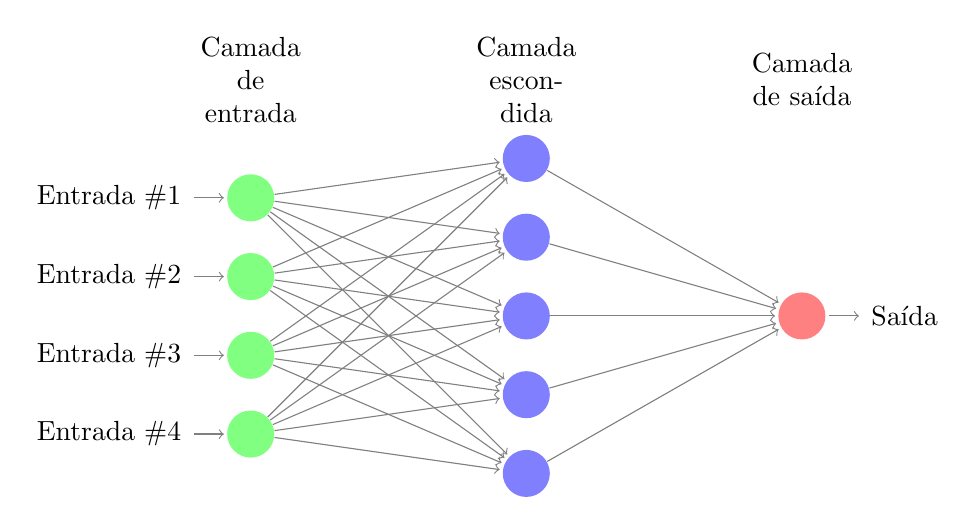
\begin{tikzpicture}[shorten >=1pt,->,draw=black!50, node distance=\layersep]
  \tikzstyle{every pin edge}=[<-,shorten <=1pt]
  \tikzstyle{neuron}=[circle,fill=black!25,minimum size=17pt,inner sep=0pt]
  \tikzstyle{input neuron}=[neuron, fill=green!50];
  \tikzstyle{output neuron}=[neuron, fill=red!50];
  \tikzstyle{hidden neuron}=[neuron, fill=blue!50];
  \tikzstyle{annot} = [text width=4em, text centered]

  % Draw the input layer nodes
  \foreach \name / \y in {1,...,4}
  % This is the same as writing \foreach \name / \y in {1/1,2/2,3/3,4/4}
      \node[input neuron, pin=left:Entrada \#\y] (I-\name) at (0,-\y) {};

  % Draw the hidden layer nodes
  \foreach \name / \y in {1,...,5}
      \path[yshift=0.5cm]
          node[hidden neuron] (H-\name) at (\layersep,-\y cm) {};

  % Draw the output layer node
  \node[output neuron,pin={[pin edge={->}]right:Saída}, right of=H-3] (O) {};

  % Connect every node in the input layer with every node in the
  % hidden layer.
  \foreach \source in {1,...,4}
      \foreach \dest in {1,...,5}
          \path (I-\source) edge (H-\dest);

  % Connect every node in the hidden layer with the output layer
  \foreach \source in {1,...,5}
      \path (H-\source) edge (O);

  % Annotate the layers
  \node[annot,above of=H-1, node distance=1cm] (hl) {Camada escondida};
  \node[annot,left of=hl] {Camada de entrada};
  \node[annot,right of=hl] {Camada de saída};
\end{tikzpicture}
\end{figure}

\subsection{Redes Neurais Artificiais para Reconhecimento de Alimentos}

Neste capítulo, são apresentados alguns dos métodos detecção e reconhecimento de alimentos através de imagens. O objetivo aqui é descrever as vantagens e principais desvantagens desses métodos e seus respectivos resultados. 


% \subsection{Detecção e Reconhecimento de Imagens}
A detecção e reconhecimento de imagens contendo alimentos são tópicos frequentemente pesquisados na área de visão computacional. Existem vários artigos publicados com diferentes abordagens para resolver esses dois problemas.  

\subsubsection{Detecção de Alimentos em Imagem}
A detecção de alimentos é diferente do reconhecimento alimentos, pois a primeira é uma classificação binária de imagens em imagens alimentares e não-alimentares, isto é, se contém comida ou não. Dada uma imagem, em que pode conter comida e fundo, a detecção de alimentos classifica a imagem como alimentar ou não-alimentar.

A Rede Neural Convolucional (CNN) oferece a mais recente técnica para muitos problemas gerais de classificação de imagem. Kagaya \cite{kagaya2014food} aplicou a CNN na classificação alimentar/não-alimentar e obteve resultados significativos com uma acurácia de 93,8\%. E, no trabalho \cite{kagaya2015highly}, a acurácia na detecção de alimentos foi aumentada para 99,1\%.

Esses resultados expressam que, em relação a trabalhos anteriores que utilizavam abordagens convencionais de aprendizado de máquina, a utilização de CNN aparenta mostrar uma melhor performance.

\subsubsection{Reconhecimento de Alimentos em Imagem}
A maioria dos trabalhos de pesquisa em reconhecimento de alimentos assumem que apenas um alimento está presente na imagem. Assim, o reconhecimento de alimentos pode ser resolvido como um problema de classificação multi-classes. 

A CNN também é amplamente utilizada no reconhecimento de alimentos e fornece melhor desempenho do que os métodos convencionais. 

Kagaya \cite{kagaya2014food} também treinou uma CNN para reconhecimento de alimentos e os resultados experimentais mostraram que a CNN superou todas as outras abordagens clássicas alcançando uma acurácia média de 73,7\% para 10 classes. Singla \cite{singla2016food} aplicou um modelo GoogLeNet pré-treinado baseado na arquitetura CNN nas tarefas de classificação de imagens alimentares/não-alimentares e para reconhecimento de categoria de alimentos. Os resultados experimentais mostram a precisão geral de 99,2\% na classificação alimentar/não-alimentar e 83,6\% na categorização de alimentos. 

A detecção e identificação de alimentos tem sido investigada na literatura em diferentes trabalhos, como os citados acima, inclusive \cite{aguilar2017food} e \cite{pouladzadeh2017cloud} em que foi evidenciado que os melhores resultados obtidos são baseados em Redes Neurais Convolucionais (CNN).



